\section{Performance evaluation}
\label{section:project_evaluation}

The implementation of Physarum-based Metaheuristic algorithm is tested under variety of conditions. Some tests have been made to show general behaviour of the algorithm depending on input problem size, while other test influence of various parameters, helping out with their selection. In the end the algorithm is compared to other common algorithms.


\subsection{Test platform}

All tests have been done on the same test machine with given specification: processor Intel Xeon E3-1246 3.5GHz, DDR3-1600 32GB RAM, Linux kernel 3.19. Same seed value has been used across the tests, unless mentioned otherwise.


\subsection{Dataset description}

bla bla bla

\subsection{Testing methodology}

\begin{figure}
  \centering

  \includegraphics[width=\textwidth]{foo.eps}

  \caption{foo bar}

\end{figure}

\begin{figure}
  \centering

  \includegraphics[width=\textwidth]{bar.eps}

  \caption{foo bar}

\end{figure}
% TODO number of plasmoida/merge number/dead number vs time -- lipa20 vs lipa90
% TODO food of each plasmodium vs time -- lipa20 vs lipa 90

% TODO scale/base
% TODO initial

% TODO various params
% TODO comparison
